\documentclass[a4paper,12pt]{article}
\usepackage[pdftex]{graphicx} 
\begin{document}

\section{}
\emph{Why do you think we didn't include error bars on the graphs in this post?}
I would guess it is because the sample size was large enough to make the standard error not worth putting on the graphs.  Since we are dealing with binary random variables the standard deviation of the sampling distribution has an upper bound of .5, which means that even if only .1\% (500/500000) of messages contained a particular target word/phrase we would still get a standard error of only 2\%.  

\section{}
\emph{The file sample\_user.csv is one user's messaging history on OkCupid. Using this data, tell me a story
about the user. I’d like as many facts as you can glean, but use your imagination, too; feel free to make
educated guesses!}

Let's approach this problem by looking at three increasingly detailed visualizations that tell the story of 6617 at increasing levels of detail.  To paraphrase one Bartholomew Simpson ``ahhh charts and graphs, statistics' only native art form. I don't count tables because they suck.''

We begin by looking at the general pattern of messages over time for 6617.  
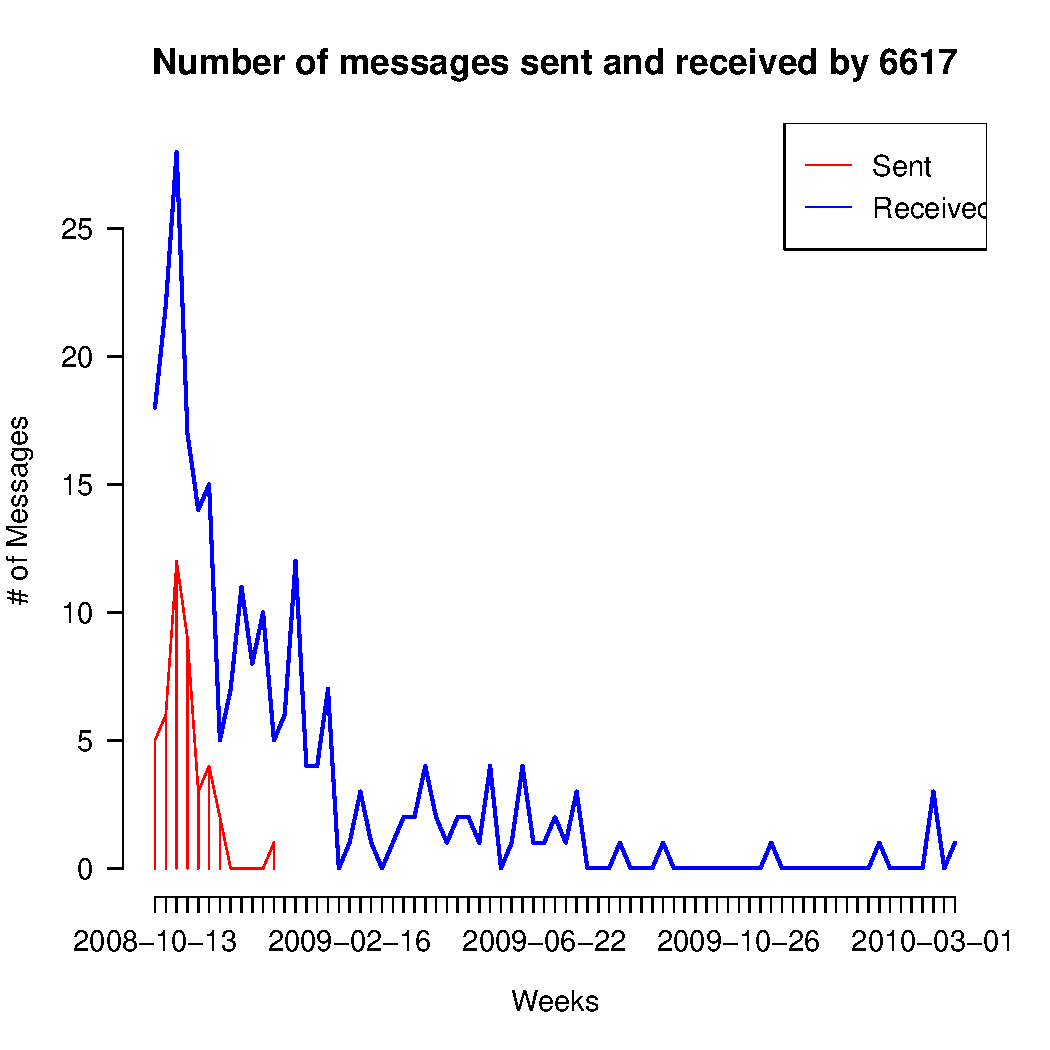
\includegraphics[scale=.75]{p2/nummess.pdf}
Our first observation is that 6617 gets way more messages than he/she sends out, we infer from this the user is female (or a wealthy attractive male) for the sake of simplicity we'll assume 6617 is female.  She also was much more active in the first few months and pretty much ceased replying to messages after the first three months, which may have caused less people to send her messages as people would have noticed her reply rate decreasing (depending on how ``replies selectively/very selectively/etc.'' determined).  From the lack of receiving activity after June we can guess 6617 not only stopped replying, but also decreased the amount she logged onto the site.   

Now that we have have a high level understanding of 6617's OkCupid usage, let's get to the good stuff: her relationships.  To get a better idea of who she was communicating with we'll examine the number of messages sent and replied to with users who had at least some interaction with 6617 (i.e. sent at least one and received at least one message).   
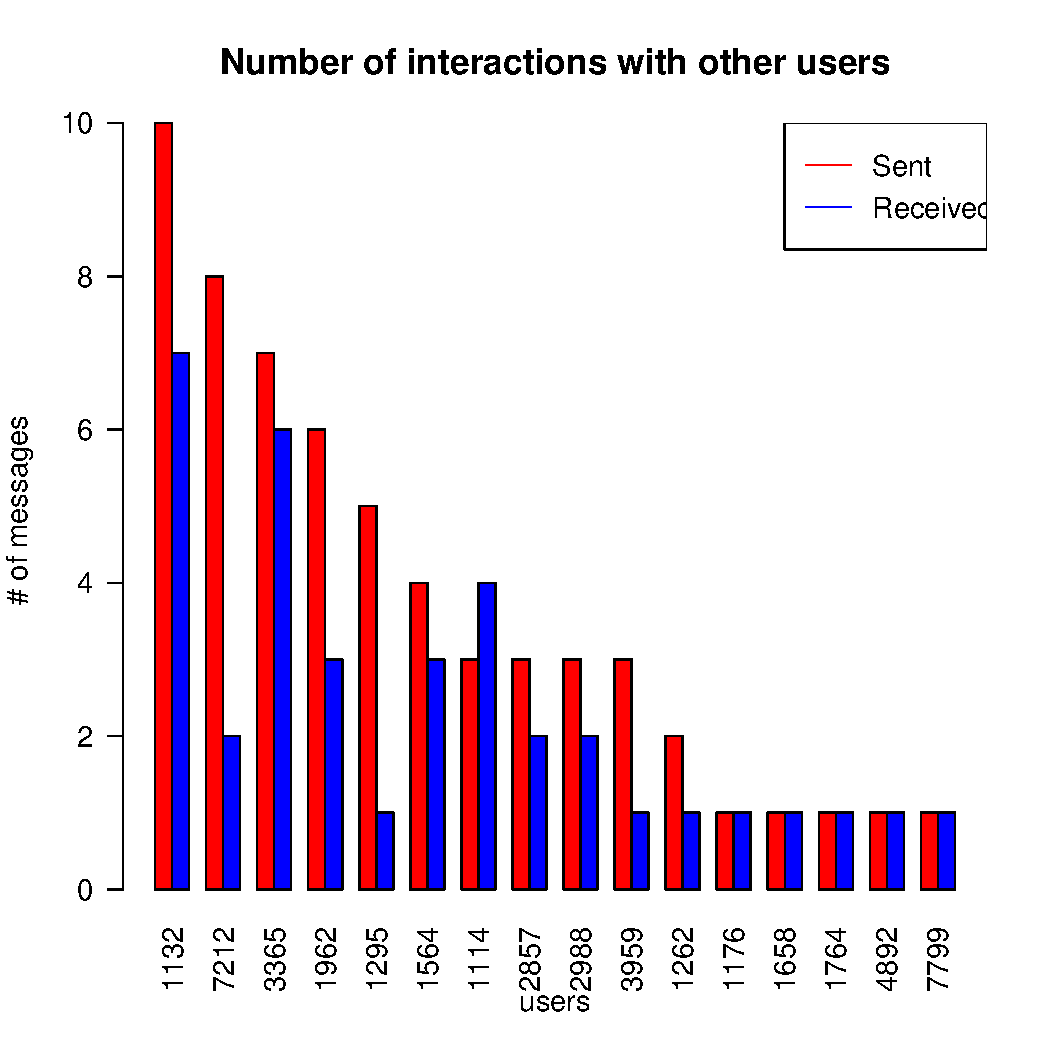
\includegraphics[scale=.75]{p2/interact.pdf}
The first thing we notice is what's not on this chart, namely the 166 unlucky souls who got nothing for their message attempts.  There were a chosen 17 who did get a message and 3 seeming ubermenschs who never wrote back.  Message patterns with individuals seems to match the global pattern of 6617 being more desired than desiring with her receiving more than sending even with the people she presumably is interested in enough to send several messages.  The main users she liked were 1132, 3365, and 1114; they not only received the most messages from 6617, but also the longest as we'll see in the next figure.  

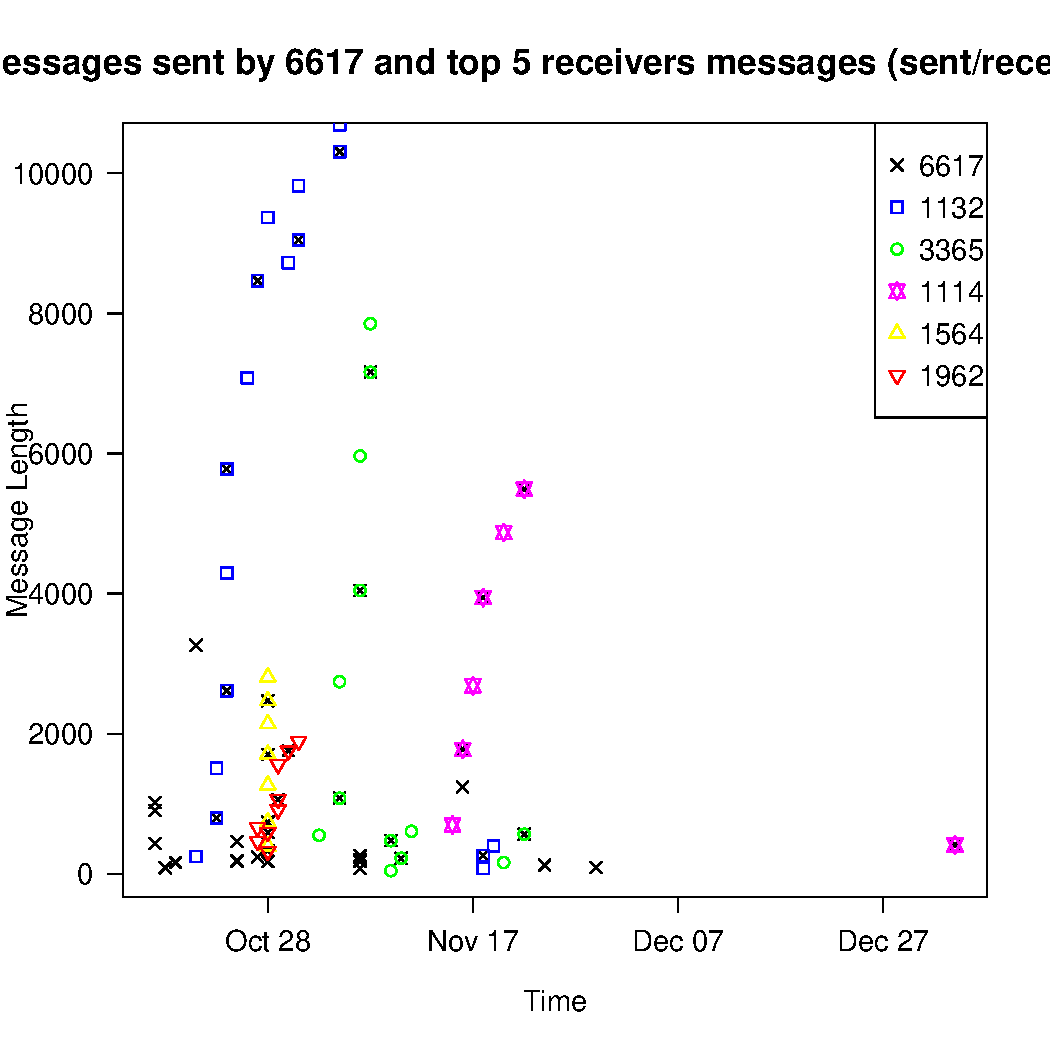
\includegraphics[scale=.75]{p2/usermess.pdf}

To get a better idea of how the indiviual interactions took place we made a scatter plot of individual messages over time with the y-axis being message length.  It looks like there's a lot going on in this graph so we'll explain it one step at a time.  The first thing to understand is the black x's represent only the messages \emph{sent} by 6617, this is different from the other marks which represent messages sent and \emph{received} for the indicated user.  What this means is when a marker, e.g. blue square, intersects with a black 'x' this represents a message that was sent by 6617 (hence the black x) to the user that corresponds with the mark, e.g. 1132 for the blue square.  Conversely marks that do not intersect a black x represent messages sent by a user to 6617.  

Now that we know what's going on we can look at the indivdual relationships that 6617 developed.  1132 was the first person to really catch 6617's eye and catch her eye he did.  1132 and 6617 had the most number of messages sent back and forth as well as 1132 receiving the 3 longest and sending the 4 longest messages to 6617.  There were a few flirtations with 1564 and 1962, but it wasn't until the appearance of 3365 that things with 1132 really changed.  Communication with 1132 pretty much ceased shortly after contact with 3365 began and a brief, but relatively involved interaction between the two started.  Things with 3365 also looked like they were evolving with longer and longer messages between the two, but it appears something happened and after a few short interchanges the two pretty much stopped talking.  After a brief cessation of activity 1114 got in touch with 6617 and there seemed to be a connection.  During this time both 1132 and and 3365 tried to get back into 6617's life, but something happened (perhaps a real life relationship with 1114) and 6617 went offline for about a month until she mysteriously sent 1114 a final message before dissapearing from the world of OkCupid forever (i.e. March 2010).

\section{}
\emph{(3) Plot a height distribution for the users in the file height.csv. This chart can contain whatever data
from the set you think is most informative, and how you display the data is totally up to you.
Remember: there is great virtue in simplicity! In addition to the chart, give me a short explanation of
your data-selection and plotting process. Some things I’d probably want to know: how did you settle on
your chart format? How did you decide how to parse the data? If you chose to exclude some segment of
the users or emphasize another, why? If you didn’t, why not? Please, generate only one chart for this
question.}

I decided to use a histogram because it seems like the most intuitive representation for a distribution of heights.  The choice to overlay different generations was made to preserve age data.  I did not find a correlation between age and height, but I felt the additional information didn't detract from getting an overall sense of the height distribution and one could infer age related facts if so desired.  The first decision was to go ahead assume this would be mainly for a US based audience.  This had two main consequences  1) the units were converted to feet/inches and 2)  age groups were generational chohorts based on how a broad sample of US citizens answered the question ``What world events are especially important to you?'' (as listed on Wikipedia's demographics page).  This meant throwing out any users over the age of 98 and while one might worry about the (almost) centenarians feeling left out, there is something to be said about being old enough to not have your generation listed in Wikipedia (to them I say enjoy your freedom from being yet another bean being counted).  I also threw out any users shorter than the shortest living person and taller than the tallest living person (i.e. anything less than 22'' and greater than 8'2'').  I binned the heights by whole inches since it is a natural unit for people to undestand height.  I considered only looking at heights within three standard deviations to get a better resolution on the mass, but I felt displaying the tails was interesting due to the assymetry of the distrubtion and most people already have a decent idea of how height is generally distributed so getting a better resolution on the center of mass didn't seem that informative.

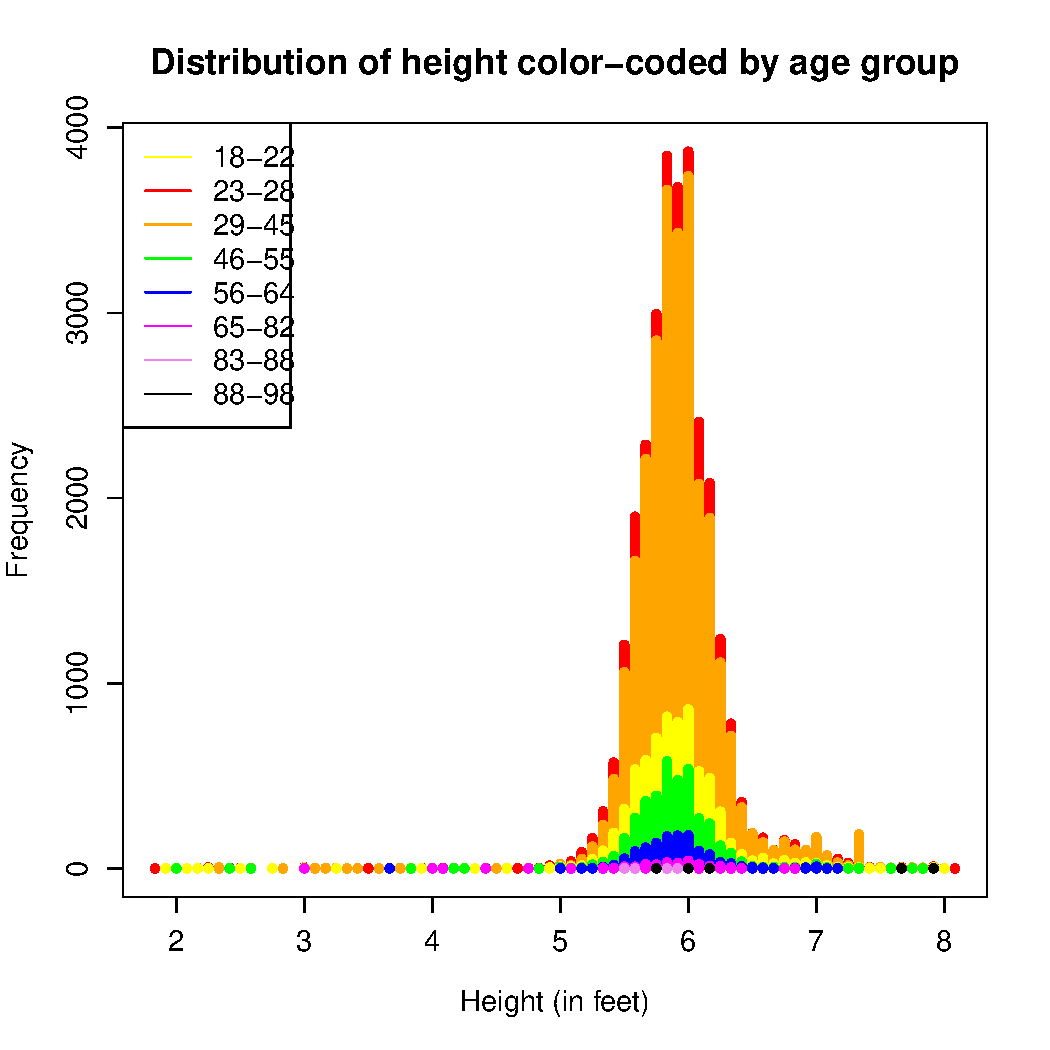
\includegraphics[scale=.80]{p3/height.pdf}
\section{}
The algorithm for finding rectangles works by finding small squares that are densely populated using a divide and conquer approcah then ``growing'' rectangles from these squares by greedily covering neighboring squares.

The 

\end{document}